%%%%%%%%%%%%%%%%%%%%%%%%%%%%%%%%%%%%%%%%%%%%%%%%%%%%%%%%%%%
% Chapter2


\pagestyle{fancy} 
\chapter{Gaussian mixture models (GMMs)}
\label{cha:2}
\vspace{1cm}

\section{Introduction}

GMM is a probabilistic model for representing normally distributed subpopulations within an overall population. Mixture models in general don't require knowing which subpopulation a data point belongs to, allowing the model to learn the subpopulations automatically. Since subpopulation assignment is not known, this constitutes a form of unsupervised learning. GMMs have been used for feature extraction from speech data, and have also been used extensively in object tracking of multiple objects, where the number of mixture components and their means predict object locations at each frame in a video sequence.

\section{Structure and Learning algorithm}
The model is parameterized by two types of values, the mixture component weights are defined as ϕk and the component means μk and variances σk or covariances (for the multivariant case) Σ, the mixture component weights has a constraint that is:  $\sum_{i=1}^{K} \phi_i = 1$ so that the total probability distribution normalizes to 1. The numerical technique used to maximize the likelihood estimation is the “Estimation maximization (EM)” which consists of tow steps:

\begin{itemize}
\item	 E-step: consist of calculating the the expectation of the component assignments $P(C_k | x_i)$ for each data point $x_i \in X$ given the model parameters $\phi_k$,  $\mu_k$, and $\sigma_k$.
\end{itemize}
\begin{itemize}
\item	M-step: which consists of maximizing the expectations calculated in the E step with respect to the model parameters. This step consists of updating the values $\phi_k$,  $\mu_k$, and $\sigma_k$.
\end{itemize}
The entire process iteratively repeats until the algorithm converges, before it starts some initializations are made as follows:
Randomly assign samples without replacement from the dataset $X={x_1, ..., x_N}$, to the component mean estimates $\mu_1, … , \mu_k$. E.g. for K=3 and N=100, set $\mu_1= x_45$, $\mu_2 = x_32$, $\mu_3 = x_10$. 
Set all component variance estimates to the sample variance 
$\sigma_1^2,...,\sigma_k^2=\frac{1}{N}\sum_{i=1}^{K} (x_i -\hat{x})^{2}=1$, where $\hat{x}=\frac{1}{N}\sum_{i=1}^{N}(x_i)$ is the sample mean.
Set all component distribution prior estimates to the uniform distribution  
$P(C_k) = \phi_1,..., \phi_k  = \frac{1}{K}$
while the E-step computes the probability that $x_i$ is generated by component $C_k$:
\begin{equation}
	 p(C_j \mid x_i ) = \frac{ p(x_i \mid C_j)p(C_j) }{p(x_i)} = \frac{p(x_i \mid C_j)p(C_j)}{\sum_ip(x_i \mid C_j)p(C_j)}
	 \label{eq:}	
\end{equation}

which will be used in the M-step where the parameters are updated as follow:	

\begin{align}
\mu_j&=\frac{ \sum_{i} p(C_j \mid x_i )x_i}{\sum_{i} {p(C_j \mid x_i )}} \\
\sigma_j^2 &=\frac{\sum_{i}{p ( C_j \mid x_i)}  (x_i - \mu_j) (x_i - \mu_j)^T} {\sum_{i} {p(C_j \mid x_i )}} \\
p ( C_j ) &= \frac{ \sum_{i} p(C_j \mid x_i )}{N}
\end{align}

\begin{figure}
\centering
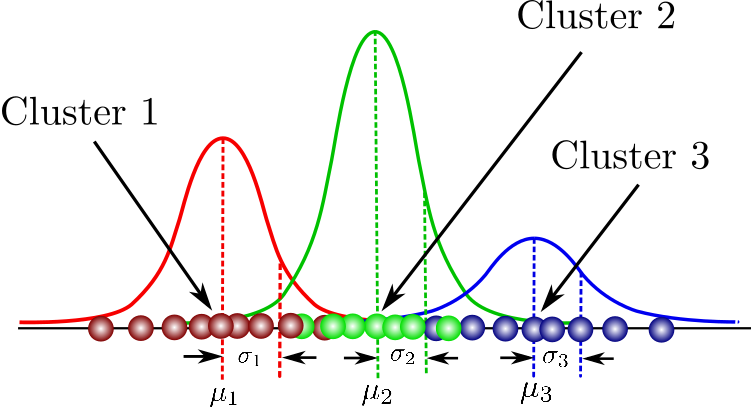
\includegraphics[scale=0.3]{Figures/GMM}
\caption{}
\label{fig:GMM}
\end{figure}

\vspace{10pt} 
Originally GMM is employed for classification and clustering tasks, but as we can deduce that it is also a suitable model when recovering the distribution of the data is needed, since it can produce more complexed distribution composed of jointed k gaussians as in Fig.~\ref{fig:GMM}, for example if we have different sources from which the data is provided. Back to our main argument, GMM has been used in several robotics applications, like in Gaussian Mixture Model for Robotic Policy Imitation~\cite{pignat2019bayesian} where different robots had to learn from few amount of demonstrations to complete various tasks such as avoid obstacles, or insert a peg in a moving hole. This approach (GMM) illustrates the advantages of learning a distribution of policies instead of trajectories and can be used in a variety of tasks. On the other hand in some work as in~\cite{zhang2016robot} the GMM was benefited in robot obstacle avoidance learning as a base for a generative model, to generate trajectories, by Gaussian Mixture Regression (GMR), The trajectory obtained not only can avoid obstacles but also can be executed by robots due to its good smooth property. The same idea of~\cite{zhang2016robot} was implemented in~\cite{reiley2010motion} in which GMM encodes the expert’s underlying motion structure. GMR is then used to extract a smooth reference trajectory to reproduce a trajectory of the task. This GMM/GMR generative model was trained on expert data, then tested by classifying the generated trajectories  to be either coming from expert, intermediate, or novice surgeons. The classification algorithm Hidden Markov Models (HMMs) trains three (expert, intermediate and novice) from five new unseen trials for each skill level. The results of the classifier show that each trajectories generated by GMM/GMR are closest to the expert model. To conclude this session it is right and proper to say that the use of GMM has remarkable impact to improve the model performance in presence of lack of data issue.


\clearpage{\pagestyle{empty}\cleardoublepage}